%% This is file `elsarticle-template-5-harv.tex',
%%
%% Copyright 2009 Elsevier Ltd
%%
%% This file is part of the 'Elsarticle Bundle'.
%% ---------------------------------------------
%%
%% It may be distributed under the conditions of the LaTeX Project Public
%% License, either version 1.2 of this license or (at your option) any
%% later version.  The latest version of this license is in
%%    http://www.latex-project.org/lppl.txt
%% and version 1.2 or later is part of all distributions of LaTeX
%% version 1999/12/01 or later.
%%
%% The list of all files belonging to the 'Elsarticle Bundle' is
%% given in the file `manifest.txt'.
%%
%% Template article for Elsevier's document class `elsarticle'
%% with harvard style bibliographic references
%%
%% $Id: elsarticle-template-5-harv.tex 159 2009-10-08 06:08:33Z rishi $
%% $URL: http://lenova.river-valley.com/svn/elsbst/trunk/elsarticle-template-5-harv.tex $
%%
\documentclass[preprint,authoryear,12pt]{elsarticle}
%% Use the option review to obtain double line spacing
%% \documentclass[authoryear,preprint,review,12pt]{elsarticle}

%% Use the options 1p,twocolumn; 3p; 3p,twocolumn; 5p; or 5p,twocolumn
%% for a journal layout:
%% \documentclass[final,authoryear,1p,times]{elsarticle}
%% \documentclass[final,authoryear,1p,times,twocolumn]{elsarticle}
%% \documentclass[final,authoryear,3p,times]{elsarticle}
%% \documentclass[final,authoryear,3p,times,twocolumn]{elsarticle}
%% \documentclass[final,authoryear,5p,times]{elsarticle}
%% \documentclass[final,authoryear,5p,times,twocolumn]{elsarticle}

%% if you use PostScript figures in your article
%% use the graphics package for simple commands
%% \usepackage{graphics}
%% or use the graphicx package for more complicated commands
%% \usepackage{graphicx}
%% or use the epsfig package if you prefer to use the old commands
%% \usepackage{epsfig}

%% The amssymb package provides various useful mathematical symbols
\usepackage{amssymb}
%% The amsthm package provides extended theorem environments
%% \usepackage{amsthm}
\usepackage{color}
\usepackage{siunitx}
\usepackage{array}

%% The lineno packages adds line numbers. Start line numbering with
%% \begin{linenumbers}, end it with \end{linenumbers}. Or switch it on
%% for the whole article with \linenumbers after \end{frontmatter}.
%% \usepackage{lineno}

%% natbib.sty is loaded by default. However, natbib options can be
%% provided with \biboptions{...} command. Following options are
%% valid:

%%   round  -  round parentheses are used (default)
%%   square -  square brackets are used   [option]
%%   curly  -  curly braces are used      {option}
%%   angle  -  angle brackets are used    <option>
%%   semicolon  -  multiple citations separated by semi-colon (default)
%%   colon  - same as semicolon, an earlier confusion
%%   comma  -  separated by comma
%%   authoryear - selects author-year citations (default)
%%   numbers-  selects numerical citations
%%   super  -  numerical citations as superscripts
%%   sort   -  sorts multiple citations according to order in ref. list
%%   sort&compress   -  like sort, but also compresses numerical citations
%%   compress - compresses without sorting
%%   longnamesfirst  -  makes first citation full author list
%%
%% \biboptions{longnamesfirst,comma}

% \biboptions{}

\journal{Biosystems Engineering}

\begin{document}

\begin{frontmatter}

%% Title, authors and addresses

%% use the tnoteref command within \title for footnotes;
%% use the tnotetext command for the associated footnote;
%% use the fnref command within \author or \address for footnotes;
%% use the fntext command for the associated footnote;
%% use the corref command within \author for corresponding author footnotes;
%% use the cortext command for the associated footnote;
%% use the ead command for the email address,
%% and the form \ead[url] for the home page:
%%
%% \title{Title\tnoteref{label1}}
%% \tnotetext[label1]{}
%% \author{Name\corref{cor1}\fnref{label2}}
%% \ead{email address}
%% \ead[url]{home page}
%% \fntext[label2]{}
%% \cortext[cor1]{}
%% \address{Address\fnref{label3}}
%% \fntext[label3]{}

% \title{An Autonomous Platform for Use in Kiwifruit Orchards}
\title{A Platform for Autonomous Navigation of Kiwifruit Orchards}

%% use optional labels to link authors explicitly to addresses:
%% \author[label1,label2]{<author name>}
%% \address[label1]{<address>}
%% \address[label2]{<address>}

% \author{Mark H. Jones, Jamie Bell, Matthew Seabright, Joshua Barnett, Alistair Scarfe, Bruce MacDonald, Mike Duke}

%% Group authors per affiliation:
\author[UoW]{Mark H. Jones\corref{mjemail}}
\cortext[mjemail]{markj@waikato.ac.nz}

\author[UoA]{Jamie Bell\corref{jbemail}}
\cortext[jbemail]{jamie977@gmail.com}
\author[UoW]{Matthew Seabright}
\author[RPL]{Alistair Scarfe}
\author[UoW]{Mike Duke}
\author[UoA]{Bruce MacDonald}

\address[UoW]{School of Engineering, University of Waikato, Hamilton, New Zealand}
\address[UoA]{Faculty of Engineering, University of Auckland, Auckland, New Zealand}
\address[RPL]{Robotics Plus Ltd, Newnham Innovation Park, Tauranga, New Zealand}

\begin{abstract}
%% Text of abstract

    We present a vehicle designed specifically for autonomous control in kiwifruit orchards.
    Here is ours and this is how it fits in with those.
    We've gone with these sensors and this method of navigation and it has demonstrated itself to work in the orchard.
    We think that we could improve the thing by using this algorithm and increasing module space.
    Generally it is an improvement on the previous work of Scarfe.

\end{abstract}

\begin{keyword}
%% keywords here, in the form: keyword \sep keyword

%% MSC codes here, in the form: \MSC code \sep code
%% or \MSC[2008] code \sep code (2000 is the default)
    Agricultural robotics \sep outdoor navigation \sep \colorbox{red}{more keywords}
\end{keyword}

\end{frontmatter}

% \linenumbers

%% main text
\section{Introduction}
\label{sect:intro}
    Short-term labor requirements within New Zealand's kiwifruit industry peak twice a year corresponding with the pollination and harvesting of kiwifruit.
    The majority of employment during these peaks is filled by seasonal or casual workers \citep{Timmins2009}.
    As kiwifruit is the country's largest horticultural export by value \citep{StatisticsNewZealand2015}, automation in this industry should promote economic growth.
    % The New Zealand government aims to double exports from its primary industries between 2012 and 2025 and is actively investing in programmes to achieve this \citep{MinistryPrimaryIndustries2015}.

    Previous work on automated harvesting of kiwifruit has been demonstrated \citep{Scarfe2012}.
    That work presents a mobile platform integrated with robotic arms that was capable of harvesting fruit from pergola style kiwifruit orchards.
    The platform presented here is a second generation unit that increases modularity by separating the platform from the tasks it performs, namely harvesting and pollination.
    This work discusses only the base platform, where details of modules for harvesting and pollination are published separately \citep{williams2017,Seabright2017}.

    Automation in kiwifruit harvesting and pollinating demands computer control, state-of-the-art manipulators, and convolutional neural networks.
    These systems are bulky and have specific geometric requirements dictated the environment and the tasks they perform.
    They share the requirements of transport to and from orchards, electrical power, and air pressure, but differ in they way they move when in the orchard.
    Pollinating modules developed as part of this project move at a well-known velocity with minimum changes in angle.
    This differs from the separately developed harvesting module that advances a set distance between stationary harvest cycles.
    The duration of such harvesting cycles are determined by the number of fruit available during any particular cycle.
    As the harvester is designed to be autonomous, there must be communication between the platform and harvester to trigger forward movement between cycles.
    Therefore, an autonomous harvesting module requires the platform it sits on to be autonomous too.

    It has been stated that ``since the robot development already includes a high complexity, the application itself should be of comparably low complexity'' \citep{Ruckelshausen2009}.
    By separating development of the base platform from the task-specific modules, risk of over-complexity is reduced by way of separation.
    The platform presented here simply needs to transport task specific modules autonomously through kiwifruit orchards.

    The development of autonomous vehicles in agriculture is not new, but much of the literature relates to existing vehicles converted to driverless.
    This work details the development of a purpose-built platform.

    \begin{figure}[htb]
        \centering
        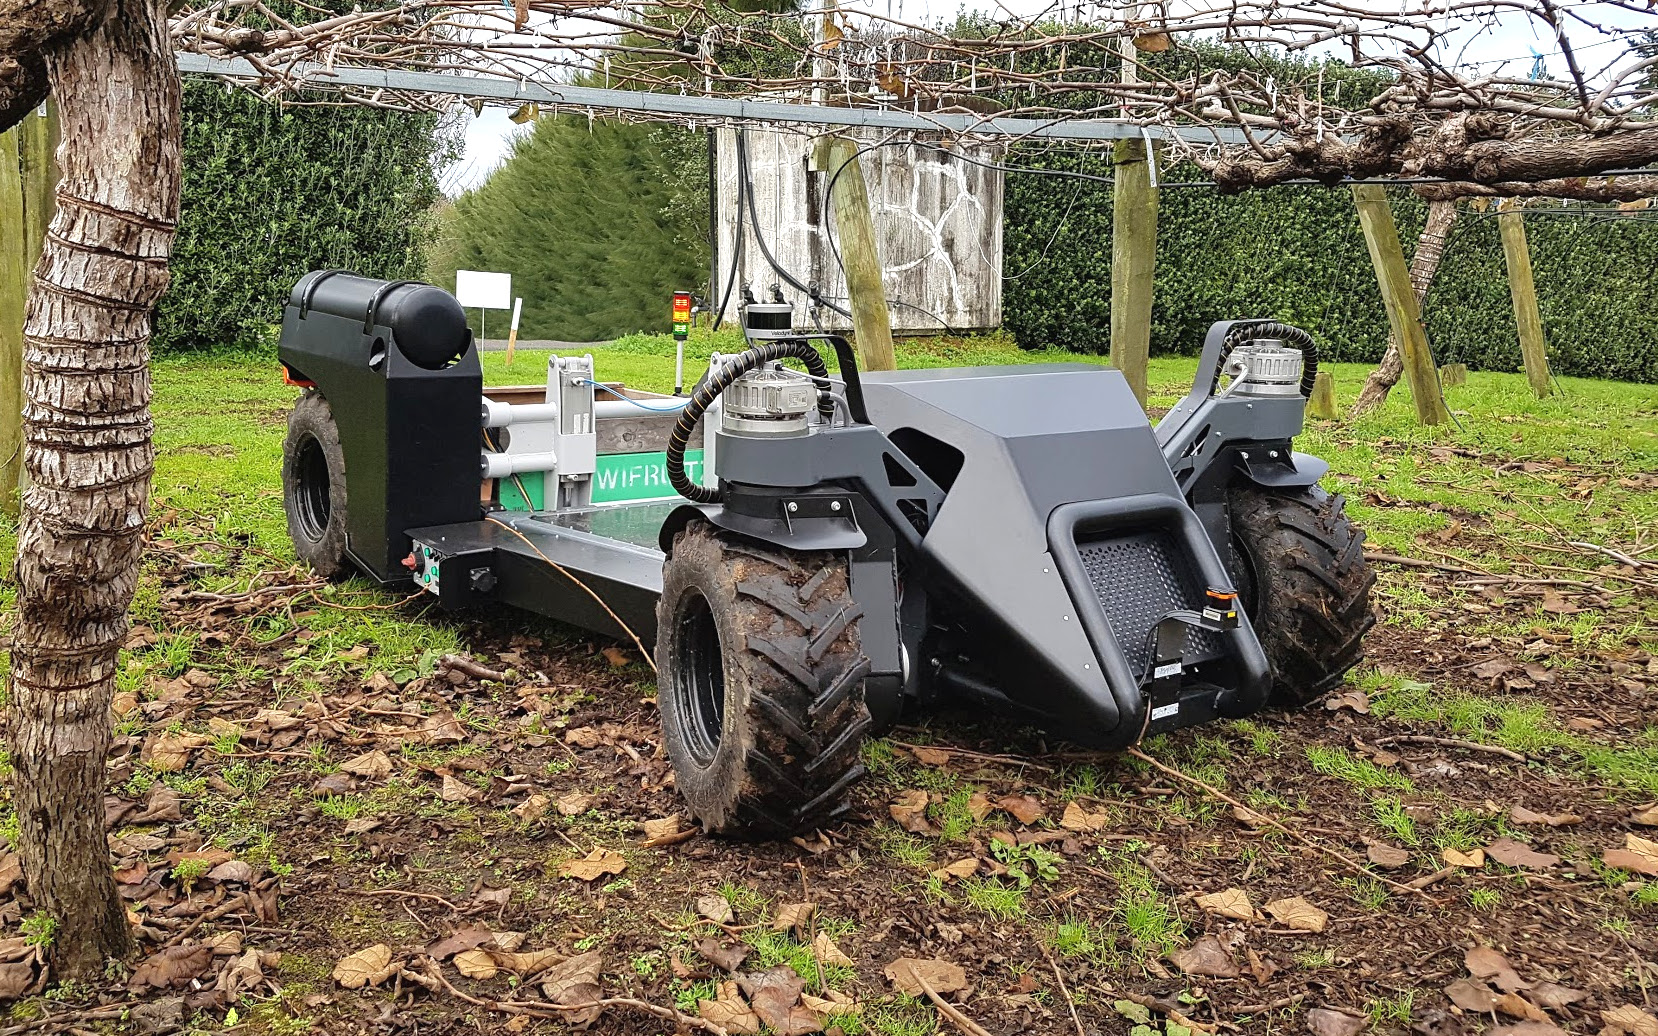
\includegraphics[width=\linewidth]{imgs/photos/suzy_general.jpg}
        \caption{
            The robot platform driving through a kiwifruit orchard.
        }
        \label{fig:suzy
}    \end{figure}

\section{Related Work}
\label{sect:review}

    \subsection{Purpose-built Autonomous Vehicles}

        The introduction of computers and digital camera technology during the 1980s sparked research into autonomous vehicles for agricultural use \citep{Li2009}.
        When publishing details of an autonomous vehicle in 1999, Tillett et~al.\@ cites difficulties dealing with variability in lighting and the environment as the reason no commercial ready vehicles were available at the time.
        Their vehicle combined wheel encoders, a compass, and accelerometers for odometry information, and featured a camera based row guidance system.
        It was capable of spraying individual plants whilst autonomously driving at a relatively slow pace of \SI{2.5}{\kilo\meter\per\hour}.

        Three years later, two autonomous robots designed for weed mapping and control were published \citep{Pedersen2002,Astrand2002}.
        These platforms had relatively simple chassis and drive systems as they were both at a prototype stage.
        They used two steering wheels and were designed specifically for field crops.
        The vehicle presented by \cite{Pedersen2002} was designed to follow pre-defined GPS based paths through row-crops, but the authors found that this was impractical without a dedicated row guidance sensor.
        Interestingly, they proposed a revised design that featured a row guidance sensor, a new drive system with four wheel steering, and utilised a Controller Area Network (CAN) bus for low level communication.
        % This work demonstrates a need to combine data from multiple sensor types.
         % Controller Area Network (CAN) bus was used to communicate with drive and steering modules on the revised unit due to it being a dominating standard in agricultural vehicles.
        \colorbox{yellow}{Did this next prototype ever get published?}

        Two years later, \cite{Bak2004} present a relatively advanced robotic platform based on a four wheel steering geometry.
        The authors noted that the control strategy for the four independently controlled wheels was non-trivial.
        Like the platform presented earlier by Pederson et~al.\@, it combined a compass, gyroscope and GPS for odommetry.
        However, it also featured a row detection sensor and a GPS receiver utilising Real Time Kinematic (RTK) corrections from a base station.
        RTK-GPS is capable of providing positioning with accuracies of around \SI{2}{\centi\meter}.
        Their robot utilised a CAN bus for some aspects of system communication.

        % In 2008, Klose et~al.\@ publish details of `Weedy', a autonomous weed control robot for field use.
        % It used an overly simple four wheel steering geometry, likely to be a cost/complexity trade-off.
        % There are few details on the sensor selection apart from mention of the use of cameras and `acoustic distance sensors'.
        % Presumably the selection of drive geometry on this robot is a cost/complexity optimisation.
        % It too makes use of a CAN bus for communication between on-board modules.

        % The following year, many the same authors appearing on the `Weedy' paper published details an autonomous robotic platform with four wheel steering named BoniRob \citep{Ruckelshausen2009}.
        After five years, in 2009, details of BoniRob are published by \cite{Ruckelshausen2009}.
        Similar to the unit presented by Bak et~al.\@ it features a gyroscope, RTK-GPS for localisation, a CAN bus for low level communication, and four wheel steering.
        What made BoniRob particularly interesting was its ability raise and lower itself and alter its wheel placement by actuating the arms to which the motors are attached to.
        Also, it introduced the use of both 2D and 3D laser-scanning (or lidar) for perception and row detection.
        % A CAN bus is used to control the low level systems (such as the drive control) and ethernet connections for higher level communication.
        The authors created a simulated model of the platform using Gazebo in which they could test the many-degrees-of-freedom drive system.
        During the previous year, some of these authors published details of a much simpler robot named `Weedy' \citep{Klose2008}.

        Of particular relevance to this work is that of Scarfe et~al.\@ on an autonomous kiwifruit picking robot \citep{scarfe2009, Scarfe2012}.
        That work involved the creation of a hydraulically driven platform with two wheel steering to which four fruit harvesting arms were integrated.
        While its ability to navigate a kiwifruit orchard was not tested, it formed the foundation for the second-generation platform we present here.

        \cite{Blackmore2007} envisaged significant reductions in production costs by re-purposing parts already in use in the agricultural and automotive industry.
        While not a physical component, the CAN is one such technology borrowed from the automotive industry aiding developmental of low-level communications.
        Many of the platforms reviewed, especially the more recent ones, made use of this protocol for real-time communication.
        Platforms designed for open field crops appear to favor four-wheel steering over two wheel steering.
        The use of simulation tools allowed the creators of BoniRob to develop and test their mobility system separate of the physical hardware.

        Common among these vehicles is the use of sensor fusion, whereby data from multiple sensors is merged and filtered.
        This provides a way to combine the advantages of multiple sensor types, and the benefit of redundancy  into a single computation space.
        With regards to the use of RTK-GPS in perception based guidance systems, Slaughter et~al.\@ points out the trade-off of requiring an ``unobstructed ``view'' of the sky from all parts of the field'' \citep{Slaughter2008}.
        Additionally, multi-path signal propagation caused by nearby foliage or the geometry of the land itself presents its own mode of failure \citep{Durrant-Whyte2005}.
        This requirement can not be satisfied under the canopy of a kiwifruit orchard which are usually surrounded by tall wind-breaking hedges.
        A separate feasibility analysis highlighted the use of RTK-GPS systems as a significant cost in yearly subscriptions alone \citep{Pedersen2006}.
        Torii suggests a combination of both RTK-GPS and machine vision systems to be the most promising system going forward based on reductions in costs and increases in performance of these systems \cite{Torii2000}.
        While \cite{Li2009} concludes that either GPS and machine vision, or GPS and lidar will be used together as a development trend.

    \subsection{Sensors for Row Based Navigation in Orchards}

        Sensors for orchard based row detection fall into two three categories; camera based, lidar based, or a combination of the two.
        The following section summarises a review of row detection efforts in orchards using these techniques.
        % Lidar come in two flavours: single-plane, and multi-layer.

        \cite{Subramanian2006} tested both camera based guidance and lidar (Sick LMS-200) based guidance systems in a citrus fruit orchard.
        Sensors were trialled separately on a tractor retrofitted with a fly-by-wire system.
        Their vehicle was able to navigate a small and simplified path using both machine vision and lidar based approaches at speeds of up to \SI{4.4}{\meter\per\second}.
        Lidar proved more accurate to the point at which the data rate became a limiting factor, after which image based approach became favourable.
        They suggest that combining the two systems would give more robust guidance as well as providing the ability to detect obstacles.
        No mention of the ability for the image based approach to cope with varying conditions is made.

        \cite{Barawid2007} demonstrate the use of data from a single-plane lidar (Sick LMS-219) being used to control a drive-by-wire tractor through an orchard.
        Their results show real-time processing of lidar data is sufficient to navigate an orchard at \SI{0.36}{\meter\per\second} (\SI{1.3}{\kilo\meter\per\hour}).

        \cite{Hansen2011} show the use of a single-plane lidar (Sick LMS-200) for vehicle localisation in an orchard.
        Also in 2011, two groups publish work on the generation of centre-lines from camera data of orchard rows.
        \cite{He2011} uses traditional machine vision, where \cite{Torres2011} makes use of neural network based image processing.
        Both methods generate valid paths, alghouth He et~al.\@ note that theirs may not be suitable when the envirnoment background becomes complex.

        The work of \cite{Scarfe2012}, combined traditional camera based image processing techniques with a single-plane lidar (Sick LMS-111).
        The image based approach failed to cope with variability in lighting conditions, however the lidar proved useful for detecting the trunks and posts of the row.

        \cite{Freitas2012} focus on the detection of people and bins in the rows of an apple orchard using lidar (Sick LMS-291), a low-cost inertial measurement unit, and wheel encoders.
        Their algorithm was capable of detecting each obstacle classe off-line from data captured in an apple orchard.

        \cite{Zhang2014} use a lidar (Hokuyo UTM-30LX) to generate maps of an apple orchard with the aid of artificial landmarks.
        They use an actuated single-plane lidar to generate multi-layer data for use in row and landmark sensing.
        Placing artificial land-marks in orchards is designed to reduce the effort required to create orchard maps for guidance systems.

        The following year, many of the same authors write about their autonomous vehicle \citep{Bergerman2015}.
        It describes a electric utility vehicle converted to fly-by-wire with the addition wheel encoders for odometry and a single-plane lidar (Sick LMS-111).
        While not able to detect obstacles in real-time, their previous work processing off-line data \citep{Freitas2012} has potential to be integrated with the addition of extra computing capability.

        Most recently, \cite{Sharifi2015} write about a method to generate a centre-line from an image an of an orchard rows.
        Like the work of \cite{He2011}, the technique offers a way to generate paths from a single camera image without resorting to neural networks.
        However, their future work focuses on increasing robustness to variations in lighting conditions, which indicates issues in this area.
        They state their system has use in being complementary to lidar based navigation.

        These works show that traditional image based processing for navigation fails when the scene becomes complex or the lighting varies.
        Combining cameras with neural network based processing increases the robustness to environmental complexities, such as light or clutter.
        The experiences of \cite{Scarfe2012} and similar indicate that Lidar outputs data which requires less post-processing to be robust.
        The use of lidar has seen two of the reported vehicles navigate autonomously through orchard environments.



\section{Platform Design}

    \subsection{Vehicle Configuration}
    \label{sect:mechanical}

        \begin{figure}[htb]
            \centering
            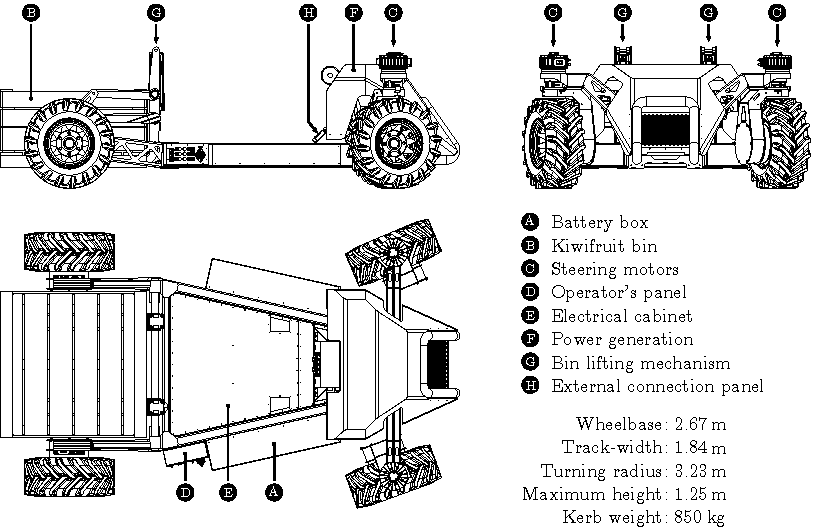
\includegraphics[width=\linewidth]{imgs/profile_views/AMMP-All-Labelled.pdf}
            \caption{Profile drawings of the robotic platform with kiwifruit bin.}
            \label{fig:AMMP}
        \end{figure}

        Modules designed to be carried by the platform require clearance from the canopy, in addition to to height they occupy themselves.
        A kiwifruit canopy ranges in height between \SI{1300}{\milli\meter} and \SI{1700}{\milli\meter}.
        To maximise space available to these modules the platform must be low-slung at the point of attachment.
        Figure \ref{fig:AMMP} illustrates the platform's design, with module area allocated between markers `F' and `E' in the side view (top left).
        The height of the chassis in this region is \SI{360}{\milli\meter} from the ground.

        Steering geometry is Ackermann based with independent motors on the front wheels for actuation.
        The ability to actuate the angles individually simplifies the mechanical geometry needed to coordinate steering, particularly at extreme steering angles.
        Steered wheels have the freedom to rotate \SI{340}{\degree}, limited by a mechanical stop.
        This range of steering angle allows the vehicle to place the centre of rotation between its rear wheels.
        At this angle, the turning circle is equal to approximately twice the length of the vehicle.
        Implementing four wheel steering would allow the centre of rotation to move to the centre of the vehicle, decreasing the turning circle to the total length of the vehicle.
        However, headlands in kiwifruit orchards are sized for tractors to turn between rows, tractors which use Ackerman steering geometries.
        The implementation of Ackermann geometry on the platform simplifies the mechanical design, removes the need to develop ``non-trivial'' control strategies, and increases the usable area.
        A differential drive, or skid steer, system was expected to cause ground damage to a level considered unacceptable to orchard owners.

        Bin lifting forks are fitted to the area between the rear wheels.
        This area is sized to accommodate a standard kiwifruit bin.
        The lifter is actuated by two vertically mounted pneumatic cylinders and is controlled by a standard pneumatic valve block.
        With this, the platform will have the ability to pick and place bins while operating in the orchard.

        Other than its tires, the platform has no suspension.
        It features a front pivoting axle that ensures that a minimum of three wheels are always in contact with the ground.
        Each wheel is mounted directly to a 40:1 fixed ratio planetary gearbox connected to a permanent magnet brushless AC motor.
        This specific gearbox-motor combination allows the platform to travel at a maximum speed of \SI{10}{\kilo\meter\per\hour}.
        The lack of suspension is not an issue when operating in orchards at this speed.
        In total, the drive system can continuously deliver \SI{25.6}{\kilo\watt} of power and \SI{3.3}{\kilo\newton\meter} of torque.
        Based on these specifications it is capable of accelerating from a stand-still to its maximum speed at an incline of \SI{20}{\degree} whilst carrying a \SI{600}{\kilo\gram} payload in \SI{2.0}{\second}.

        A power generation unit including a petrol engine, air compressor, and alternator is fitted at the front of the vehicle.
        The drive shafts of each are connected by a heavy-duty timing belt.
        The compressor and alternator are activated electronically by an embedded controller module.
        Fuel and compressed air tanks sit over the right-hand rear wheel, these can be seen in figure \ref{fig:suzy}.
        Battery modules attached to the sides of the chassis each house fifteen lithium-iron-phosphate batteries (thirty batteries in total).

        Unloaded, the machine has an estimated mass of \SI{850}{\kilo\gram}, including the power generation unit.
        It is capable of carrying a \SI{1000}{\kilo\gram} payload.
        The mass of a standard bin of kiwifruit can be as much as \SI{400}{\kilo\gram}, leaving \SI{600}{\kilo\gram} for modules.
        % With that load, the platform's maneuverability and ability to brake or accelerate was not noticeably affected.


\section{Navigation Sensors}
\label{sect:sensors}
    The choice of sensors incorporated into a platform determines which approaches are available for navigation and object detection.
    This section details the sensor selection specific for use in kiwifruit orchards.
%     Sensor selection was a critical early step in the development of the navigation system for the AMMP because it dictated the direction of subsequent research. Four approaches were used in the process of sensor selection:
%     \begin{enumerate}
%         \item Conducting a literature survey of sensors previously used in orchard navigation and similar applications.
%         \item Surveying the features, specifications and cost of sensors available to purchase in order to perform a cost-benefit analysis.
%         \item Purchasing some sensors, based on the cost-benefit analysis, collecting data from the sensors in kiwifruit orchards and analysing the data to ensure that the sensors perform according to some minimum criteria in the orchard environment.
%         \item Developing simple algorithms for the sensor data to demonstrate that the sensors can perform the functions that they have been purchased for.
%     \end{enumerate}

% \subsection{Sensor Literature Survey}
%     From the existing literature, it seems that the existing sensors that have been commonly used for orchard navigation systems are cameras, 2D lidar, GPS, inertial sensors and encoders for odometry. Some examples are summarised in Table \ref{table:1}.

%     \begin{table}[h!]
%     \caption{Examples of sensors used in previous orchard navigation research.}
%     \centering
%     \begin{tabular}{ | m{3.2cm} | m{3.2cm}| m{6.2cm} | }
%     \hline
%     \textbf{Reference} & \textbf{Application} & \textbf{Sensors} \\
%     \hline
%     Subramanian et al., 2006 & Citrus grove navigation & Angled down 2D lidar and camera (640x480) separately; steering encoder \\
%     \hline
%     Barawid et al., 2007 & Autonomous tractor & Horizontal 2D lidar \\
%     \hline
%     Hansen et al., 2011 & Autonomous orchard vehicle & Horizontal 2D lidar, fibre optic gyroscope, odometry (encoders) \\
%     \hline
%     He et al., 2011 & Orchard row detection & Camera (640x480) \\
%     \hline
%     Torres- Sospedra and Nebot, 2011 & Orchard row detection & Camera (640x480) \\
%     \hline
%     Scarfe, 2012 & Kiwifruit harvesting robot & Horizontal 2D lidar, fluxgate compass \\
%     \hline
%     Freitas et al., 2012  & Orchard robot obstacle detection & Angled down 2D lidar, wheel and steering encoders, low cost IMU \\
%     \hline
%     Zhang et al., 2013  & Orchard robot row following & Rotated 2D lidar; lidar rotation, wheel and steering encoders \\
%     \hline
%     Bergerman et al., 2015 & Autonomous orchard vehicle & Horizontal 2D lidar, wheel and steering encoders \\
%     \hline
%     Bargoti et al., 2015 & Apple orchard localisation & Vertical 2D lidar, Global Positioning Inertial Navigation System \\
%     \hline
%     Jagbrant et al., 2015 & Almond orchard localisation & Vertical 2D lidar, Global Positioning Inertial Navigation System \\
%     \hline
%     Sharifi and Chen, 2015 & Orchard row detection & Camera \\
%     \hline
%     \end{tabular}
%     \label{table:1}
%     \end{table}

\subsection{Sensor Selection}

    As the drive motors have built-in wheel encoders, odometry data is already available on the platform.
    Encoders from powered wheels give false readings if wheel slip occurs, so these sensors cannot be used for odomentry alone.
    The data they provide can be used to assist with mapping, localisation, and provide velocity feedback.

    \begin{table}[htbp]
        \centering
        \footnotesize
        \begin{tabular}{ l l}
            \textbf{Sensor Type}      &\textbf{Possible Issues} \\ \hline
            GPS receiver              & Prone to signal loss from surrounding foiliage\\  \hline
            Inertial Measurement Unit & Error accumulation and thermal drift\\ \hline
            Digital Compass           & Can be affected by nearby metal structures\\ \hline
            Encoder                   & Error accumulation \\ \hline
            Lidar                     & Reduced visibility in fog and heavy rain \\ \hline
            Time of Flight Camera     & Reduced visibility in sunlight, fog and heavy rain \\ \hline
            Camera                    & Reduced visibility in fog or direct sunlight \\ \hline
            Thermal Camera            & Reduced visibility in conditions of low thermal contrast\\ \hline
        \end{tabular}
        \label{table:sensor_comparison}
        \caption{Sensor types considered for inclusion on the platform.}
    \end{table}

    Other sensors considered for inclusion, and their associated issues, are outlined in table \ref{table:sensor_comparison}.
    Factors influencing which sensors were trialled were the benefits and issues of each sensor, reported usage in literature for similar environments, and availability at a commercially viable price.
    The investigation suggested that lidar, and cameras offered the most functionality for navigation and object detection.
    Time-of-flight were a compelling option based on the cost-benefit analysis; especially if the less expensive units work in sunlight.
    Because localisation is such a key functionality, the performance of GPS has been evaluated in a kiwifruit orchard.
    The following sections detail our experiences while trialling these sensors.

% \subsection{Data Collection and Inspection}
 %    The sensors that seemed important to test, based on both the literature survey and the cost-benefit analysis were lidar, cameras and GPS.
	% In addition, time of flight cameras were considered, because they seemed to be a compelling option based on the cost-benefit analysis; especially if some of the less expensive models were found to work well in sunlight.
	% It was also decided that encoders would be tested in favour of using an IMU because the encoders were built into the AMMP motors.
	% Some data was collected from each sensor in order to decide which sensors to prototype algorithms for.

    \subsubsection{In-orchard GPS Evaluation}
        Two GPS modules were evaluated: a Ublox Neo-M8N module and an OmniSTAR 5120VBS with AX0 series antenna.
    	Both were connected via serial to a Beaglebone Black single board computer for data acquisition.
        The Ublox module was selected for its -167 dBm sensitivity, internal Low Noise Amplifier (LNA), and active circuitry for the 25mm square ceramic patch antenna.
        The OmniSTAR receiver was chosen for its high gain antenna (34 dB) which claims high multi-path rejection.

        The testing procedure first involved planning a path through a single row within a kiwifruit orchard and plotting it on a satellite map.
        Waypoints were placed along the row at the location of posts used to hold the canopy structure.
        Relative distances between these waypoints was measured with a tape measure and recorded.
        The receivers were then tested separately, one after the other.
        Before testing, each unit was powered up and given \SI{30}{\minute} to initialise in an open area near the kiwifruit orchard.
        During the test, each unit was walked slowly through the pre-determined path with stops at each of the waypoints to provide time for a fix.
        The path of approximately \SI{500}{\meter} took approximately \SI{15}{\minute} to complete, including stops at each waypoint.
        Waypoints were spaced approximately every \SI{5.5}{\meter} along the selected orchard row.

        \begin{figure}[htb]
            \centering
            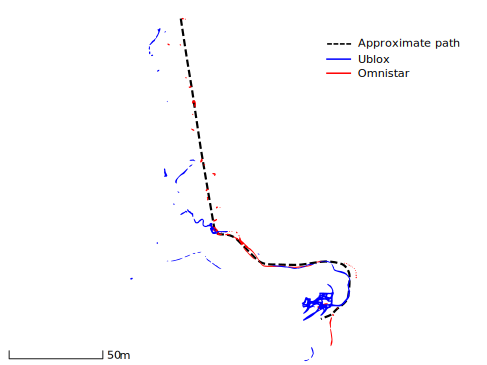
\includegraphics{imgs/gps_path/gps_path.pdf}
            \caption{
                Aerial view of a path through a kiwifruit orchard and the associated GPS data.
            }
            \label{fig:gpsResults}
        \end{figure}

        The path followed and the corresponding GPS locations collected from the receivers is presented in figure \ref{fig:gpsResults}.
        It should be noted that data has been recorded for the round-trip, so represents two passes along the path.
        It was noticed during testing that the signal quality lights on both GPS receivers regularly indicated a loss of signal.


        The Omnistar receiver appears to track the approximate path well, but the data is sparse with regular loss of signal when in the orchard.
    	The Ublox receiver collected more data than the Omnistar unit, but was much less accurate.
        It may be possible to use a unit such as the Omnistar, which provided more accurate but fewer readings, as a sanity check for an approximate location within an orchard.
        Overall the units could not be relied on for localisation under the kiwifruit canopy and were not used for navigation.

    \subsubsection{In-orchard Lidar Evaluation}
        Three lidar were evaluated, two single-plane lidars and one multi-layer lidar.
        The two single-plane lidars were the Hokuyo UTM-30LX and a SICK LMS111.
        The multi-layer is a Velodyne VLP-16 which has 16 horizontal \SI{360}{\degree} planes spread over \SI{15}{\degree}.
        Data was collected from each lidar by driving through orchard rows with the sensor placed midway between the ground and canopy (approximately \SI{0.8}{\meter} off the ground).

        \begin{figure}[htb]
            \centering
            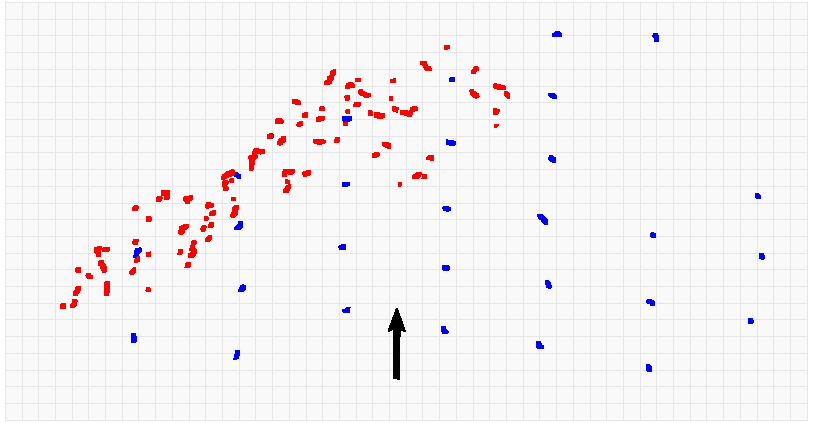
\includegraphics[width=\linewidth]{imgs/canopy_data/canopy_data.pdf}
            \caption{
                Captured lidar data showing the points reflected by the canopy (indicated by red markers) and points from tree trunks and posts (green markers).
                The arrow indicates the position and heading of the platform.
            }
            \label{fig:canopyDataCloud}
        \end{figure}

        The intention was to use the lidar as a means of detecting structure defining features of the orchard, such as posts, trunks and hedges.
        Detecting these features should allow for row boundary detection, or general mapping and localisation.
        However, both single-plane lidar produced clouds of unstructured data amongst the structured features, as shown in Figure \ref{fig:canopyDataCloud}.
        This was caused by the lidar's scan plane intercepting with the canopy on convex slopes.
        Similarly this issue arose on concave slopes where the plane intercepted with the ground, as depicted in figure \ref{fig:concaveSlope}.

        \begin{figure}[htb]
            \centering
            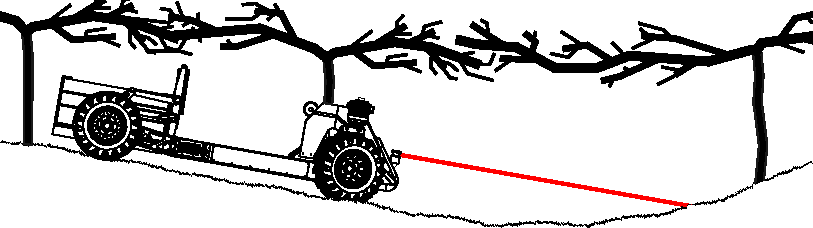
\includegraphics[width=\linewidth]{imgs/concave_slope/concave_slope_v4.pdf}
            \caption{
                On concave slopes the lidar scan plane intercepts with the ground instead of trunks or posts.
            }
            \label{fig:concaveSlope}
        \end{figure}

        This issue can be reduced when using a multi-layer lidar.
        Because of the 16 layers, it is possible to select the scan layer that gives the longest viewing range.
        Referring to figure \ref{fig:concaveSlope}, that would correspond to a layer above the horizontal.

        In this environment a single-plane liadr could still be used at relatively short range as an independent channel of processing for redundancy or obstacle detection.
        It was decided that a multi-layer lidar would be best suited for navigation due to its ability to to see longer changes on undulating ground in kiwifruit orchards.
        For the platform, a single-plane lidar has been fitted to the front of the vehicle an object detector for possible collisions, and a multi-layer lidar has also been fitted for use in navigation and general object detection.


    \subsubsection{In-orchard Camera Evaluation}
        \label{sect:camera_evaluation}

        Three varieties of camera were tested: time-of-flight, 3D stereoscopic, and traditional colour camera.

        The time-of-flight based camera was the Basler TOF640-20GM-850NM.
        It provides both depth and return signal data at a resolution of 640 by 480 pixels.
        This model was chosen for testing as it had previously proved useful when collecting depth data of kiwifruit canopies.
        During those usages it was operated under different lighting conditions and exhibited minimal occurrences of data washout.
        However, these tests revealed that in both direct sunlight and overcast conditions there was significant data loss.

        The 3D stereo camera tested was an Intel RealSense R200.
        It combines a stereo pair of infra-red cameras with a colour camera.
        Additionally, it features an infra-red projector as a means of adding ``texture'' to objects in its field of view to assist with stereo processing.
        The appealing characteristics of this sensor were its low cost and its claim as being long-range and able to work outdoors.
        However, in overcast and sunny conditions, it suffered from a complete loss of range data.

        Finally, traditional colour cameras trialled were the Basler Dart daA1600-60uc, Flir CM3-U3-13S2C-CS, and Logitech C920 cameras.
        The cameras were driven through the orchard at a height of \SI{0.8}{\meter} from the ground.
        The Logitech C920 cameras suffered from significant motion blur.
        In addition, these cameras did not provide a hardware trigger interface, which would be important if the cameras were used in stereo vision applications.
        The Basler and Flir cameras both produced images of sufficient quality.
        The Basler offering was favored for its later model image sensor.

        Overall, colour camera images were the best suited for object detection and classification.
        This is verified by processing the data using readily accessible detection algorithms.

\subsection{Sensor Demonstration by Prototype Algorithm}

    Basic tests indicated that multi-layer lidar and colour camera sensors were best suited as primary navigation sensors.
    Further testing by prototyping navigation algorithms was made to ensure the apparent sensor benefits translated into practical advantages.
    The goals for the navigation system are:

    \begin{itemize}
        \item object detection and classification,
        \item mapping and localisation, and
        \item row tracking.
    \end{itemize}
    To validate that the sensors could perform these functions, prototype navigation algorithms have been created.

    \subsubsection{Object Detection and Classification}

        % Object detection and classification was firstly prototyped fully on the camera data.
        Based on existing success using Convolutional Neural Networks (CNN) for image processing tasks \citep{LeCun2015}, a camera based system was chosen for object detection and classification.
    	The network architecture chosen was FCN-8s \citep{long2015}.
        It is a neural network made of convolutional layers without fully connected layers.
        % convolutional layers at the input and fully connected layers at the output.
    	FCN-8s performs semantic segmentation, which is per pixel labelling of images.
        To train the FCN-8 network, the camera image dataset used to assess the camera performance in section \ref{sect:camera_evaluation} was hand labeled.
        % , which was created in order assess the cameras for sensor selection, was reused and hand labelled.
    	Labeling involved drawing object outlines in each image, filling those outlines with colours corresponding to the object type, and filling any non-labeled areas with black.
        The resulting image was then converted to a palleted indexed format.
    	An example of an original image and a corresponding label image is shown as figure \ref{fig:segImgLabelPair}.

        \begin{figure}[htb]
            \centering
            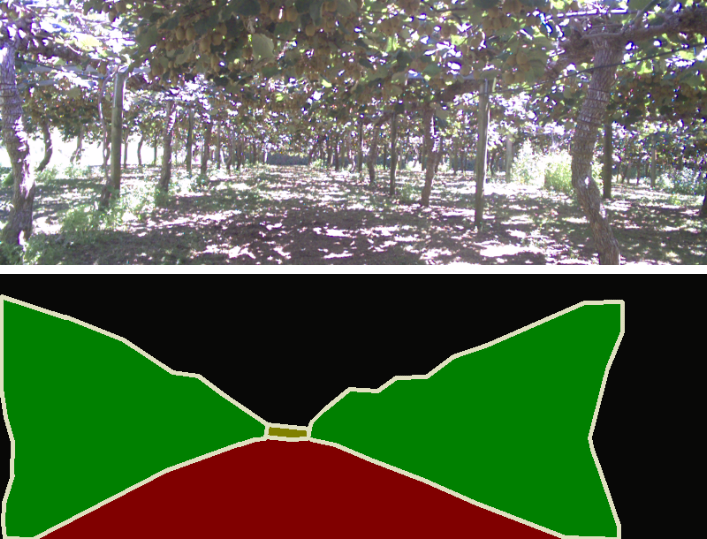
\includegraphics[width=\linewidth]{imgs/photos/segImgLabelPair_trimmed.png}
            % \includegraphics[width=\linewidth]{imgs/photos/segImg_sideBySide.png}
            \caption{
                An input image (top) and labelled output (bottom) for semantic segmentation.
            }
            \label{fig:segImgLabelPair}
        \end{figure}

        \begin{figure}[htb]
            \centering
            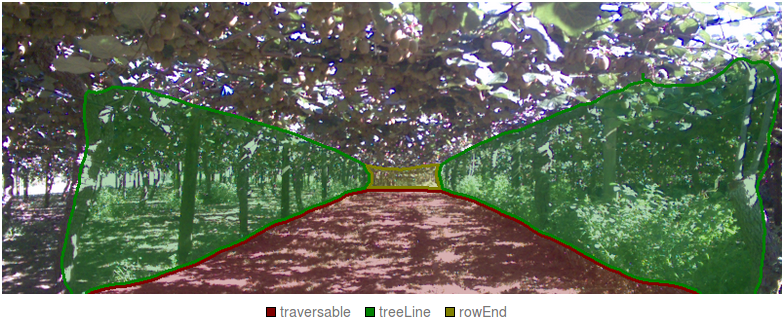
\includegraphics[width=\linewidth]{imgs/photos/semSegRowResults.png}
            \caption{
                An example result from the FCN-8 network, segmenting a kiwifruit orchard row.
            }
            \label{fig:semSegRowResults}
        \end{figure}

        Experimentation with labelling individual trees and posts in the kiwifruit orchard was performed.
    	However, labeling the entire treeline as a single class gave the best results.
    	Objects labeled during algorithm prototyping were:
        \begin{enumerate}
        \item traversable space (labeled as red),
        \item treelines (labeled as green), and
        \item the end of the row (labeled as tan).
        \end{enumerate}
        Traversable space was defined as the ground area that the platform could drive directly to without collision.
        These labelled images were then used to train the FCN-8 network.
    	Sample output from the trained network is presented as figure \ref{fig:semSegRowResults}.

    \subsubsection{Mapping and Localisation}
        An existing Simultaneous Localisation and Mapping (SLAM) package was used to test the multi-plane lidar.
        The package was Gmapping \citep{Grisetti2007}, implemented as a ROS package \citep{Gerkey2010}.
    	Required input for Gmapping is odometry data and a single plane of lidar data.
        The obometry data was provided by the platforms built-in wheel encoders and the Velodyne VLP-16 lidar was used as the lidar.
    	As this lidar has 16 scanning layers, a conversion was performed to produce the single plane of lidar data required by Gmapping.
        The easiest conversion would by to simply select a single plane from the 16 available layers and discard the remaining data.
        However, by taking this approach the system would loose any benefit offered by the multiple scanning layers.
        This would then produce the unstructured clouds of data observed with the single-plane lidar.
        Instead, a point filtering approach was used.

        \begin{figure}[htb]
            \centering
            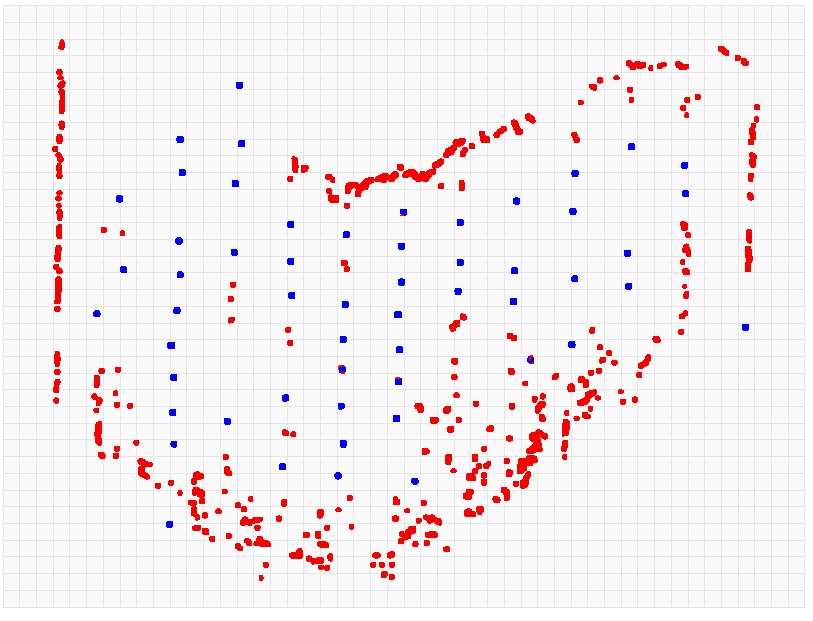
\includegraphics[width=\linewidth]{imgs/single_plane_extraction/single_plane_extraction.pdf}
            \caption{
                Processing of multi-layer lidar data into a single plane equivalent.
                Blue points are those selected by the algorithm for further processing, whereas red are rejected.
            }
            \label{fig:singlePlaneExtraction}
        \end{figure}

        Filtering the multi-layer data into a single plane was done by examining data from the centre four layers at each azimuth.
        If the difference between all four points is below a certain threshold, the closest point is returned.
        Alternatively, if the spread in points is above the threshold, no points are returned.
        This has the effect of eliminating points returned from the ground or canopy when driving over concave or convex ground, while still returning information about the location of posts and branches.
        The resulting points are then fed into Gmapping as a single plane of data along with the platform's wheel encoder data.

        \begin{figure}[htb]
            \centering
            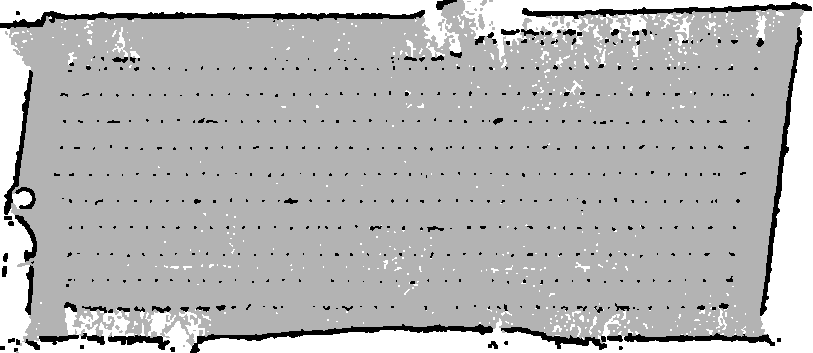
\includegraphics{imgs/gmapmap/gmapmap.pdf}
            \caption{
                A resulting SLAM based map of a kiwifruit orchard created using Gmapping.
                Odometry information has been taken from wheel encoders and a multi-layer lidar.
            }
            \label{fig:gmapmap}
        \end{figure}

        Figure~\ref{fig:singlePlaneExtraction} shows the ability of this method to filter structure data from canopy or ground reflections.
        Using this method, a SLAM based map of the orchard was created by driving the lidar through only four of the orchard's rows, presented as figure \ref{fig:gmapmap}.


    \subsubsection{Kiwifruit Orchard Row Tracking}
        \label{sect:row_tracking}

        The last navigation test requires interpreting the orchard's structure and generating a path based on that structure.
        Using the single-plane lidar data extraction technique used previously for SLAM mapping, a row guidance system is tested.
        Details of the algorithm used for row navigation have been published elsewhere \citep{Bell2016}.
        The key part of this algorithm was the calculation of the angular offset of the robot’s coordinate system from the row centreline.
        Data captured while the platform navigated the kiwifruit orchard is presented as figure \ref{fig:lastLidarFrame}.

        \begin{figure}[htb]
            \centering
            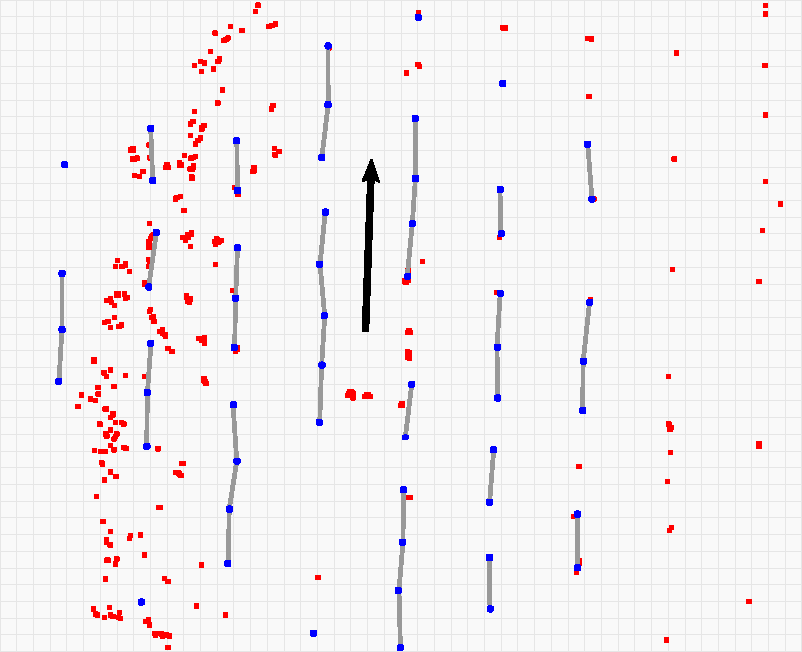
\includegraphics[width=\linewidth]{imgs/row_following/row_following_narrow.pdf}
            \caption{
                Row detection from multi-plane lidar data.
                Red points indicate non-structured data that have been ignored.
                Blue points indicate orchard structure data used for row navigation.
                Grey lines link orchard structure points by their nearest neighbours.
                The black arrow represents the centreline of the row current row.
            }
            \label{fig:lastLidarFrame}
        \end{figure}

        Row following was performed by calculating the steering angle from the sum of the proportional control signals for the linear and angular offsets of the robot from the row centreline.

        % A 3D lidar navigation algorithm was developed and tested on smaller robot platforms, as described by Bell et al. \citep{Bell2016}.
        % The key part of this algorithm was the calculation of the angular offset of the robot’s coordinate system from the row centreline.
        % This algorithm attempted to extract the posts and trees from the lidar data and then find the angle between posts and trunks in the same treeline. The key steps of the algorithm were:
        % \begin{enumerate}
        % \item Clusters of close consecutive points were found in each plane of the 3D lidar data using the method described by Scarfe [24]⁠.
        % \item Clusters with a length greater than a threshold were deemed to be unlikely to be row defining features, such as posts or trunks; as a result, these clusters were removed.
        % % \item Any clusters within a set distance of a set number of other clusters were also removed because these clusters could be a part of the clouds of data, which are returned from non structure defining features such as the kiwifruit canopy or the ground. An example result after this step for a single plane of the 3D lidar data is shown in Figure \ref{fig:singlePlaneExtraction}.
        % \item The clusters from multiple planes were grouped based on a threshold distance between clusters.
        % \item The heights of the resulting groups from step 4 were compared to a threshold to determine which were posts and trees. An example result after this step for a single frame of 3D lidar data is shown in Figure \ref{fig:lastLidarFrame}.
        % \item Using the data from feature extraction, each cluster’s nearest neighbour was found. This step was taken because most posts and trunks are closer to other posts or trunks in the same tree-line than to an adjacent tree-line. This suggests that the angle between nearest neighbours should also be the angle of the tree-line.
        % \item Nearest neighbours that were further apart than the row width were rejected to eliminate the possibility of using neighbours that were not in the same tree-line.
        % \item The angles between the resulting nearest neighbours were calculated.
        % \item The mode of the calculated angles was taken to be the current estimate of the angular offset of the robot from the row centreline.
        % \end{enumerate}

        % Once the angular offset was found, the linear offset of the robot’s coordinate system origin from the row centreline was calculated. The steps used were:
        % \begin{enumerate}
        % \item The clusters belonging to the current row were found using the angular offset and the maximum row width for the orchard.
        % \item Lines were fitted to the treelines on the left and right sides of the row.
        % \item The row centreline was found as the average line from the left and right treelines.
        % \item The displacement of the robot centre from the row centreline was calculated.
        % \end{enumerate}

        % Row following was performed by calculating the steering angle from the sum of the proportional control signals for the linear and angular offsets. Row end detection was performed by detecting a volume of free space above the 3D lidar sensor. Row end driving was performed by driving a sequence of set curvature movements, while performing obstacle avoidance.

        % The autonomous driving algorithm described here has been used to drive 20 km autonomously on three different robot platforms, including the AMMP, in two different real kiwifruit orchards. This driving was performed using just lidar and encoder data.

        % \begin{figure}[htb]
        %     \centering
        %     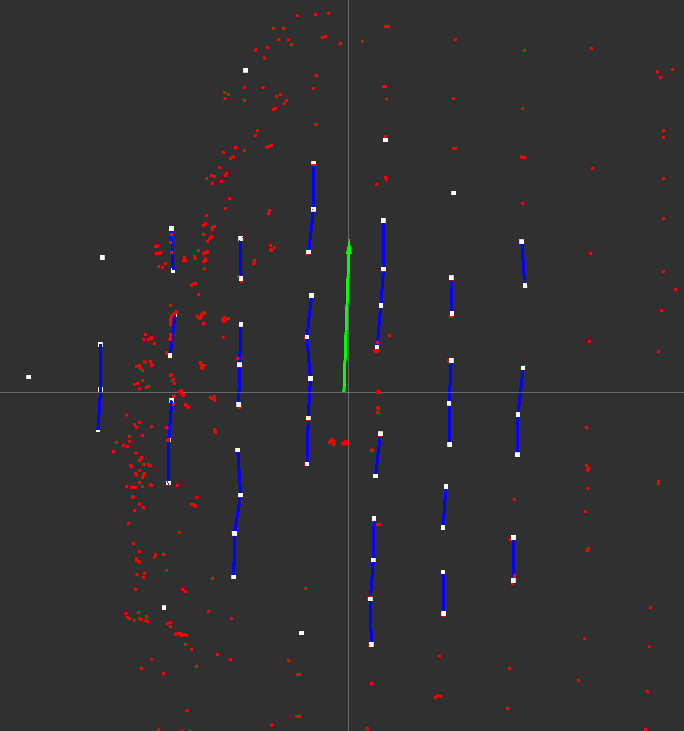
\includegraphics[width=\linewidth]{imgs/photos/lastLidarFrame.png}
        %     \caption{
        %         A single plane of 3D laser scanner data (red) with the points found by feature extraction highlighted in white, nearest neighbours indicated with blue and the detected row centreline (green arrow).
        %     }
        %     \label{fig:lastLidarFrame}
        % \end{figure}

\subsection{Sensor Selection Conclusions}
    The results from prototyping algorithms indicate that the 3D lidar and encoder sensors may be feasible selections for performing mapping, localisation and autonomous driving in kiwifruit orchards.
	Object detection using cameras in kiwifruit orchards is also possible.
	Given these results with prototyping algorithms for the navigation system, it was decided to proceed with using cameras, 3D lidar and encoders as the primary sensors for the navigation system.
    The autonomous driving algorithm described here has been used to drive 20 km autonomously on three different robot platforms, including the AMMP, in two different real kiwifruit orchards. This driving was performed using just lidar and encoder data.



\section{System Architecture}
\label{sect:hardware}

    \newcommand{\rpm}{\raisebox{.2ex}{$\scriptstyle\pm$}}

    \begin{figure}[htb]
        \centering
        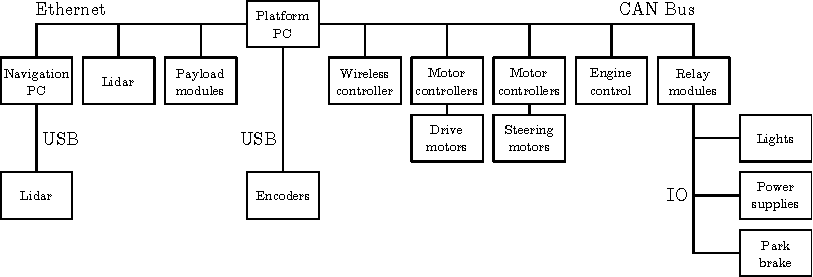
\includegraphics[width=\linewidth]{imgs/system_diagram/diagram_v3.pdf}
        \caption{Hardware level system diagram showing the types of interfaces and relative relations on the platform.}
        \label{fig:system_diagram}
    \end{figure}
    Sub-systems on the platform, including the drive system, are connected to the system PC via a CAN bus, as shown in figure \ref{fig:system_diagram}.
    The CANopen protocol has been implemented which offers message type prioritisation and a standardised way of sharing process data.
    Messages on the bus during operation are restricted to commands, syncronisation messages, and status updates.
    Relay modules connected to the bus allow the system to control the power to its on-board power supplies, motor controllers, park brakes, and lights.
    They also monitor the timing of synchronisation messages transmitted by the system PC and will enter an error state if the timing falls outside set limits.
    These messages must be transmitted every \SI{20}{\milli\second}, with a maximum allowable error of \rpm \SI{5}{\milli\second} \colorbox{red}{check these figures}.
    Entering an error state results in the motor controllers being disabled, park brakes engaged, and power to the power supplies being cut.

    \begin{figure}[htb]
        \centering
        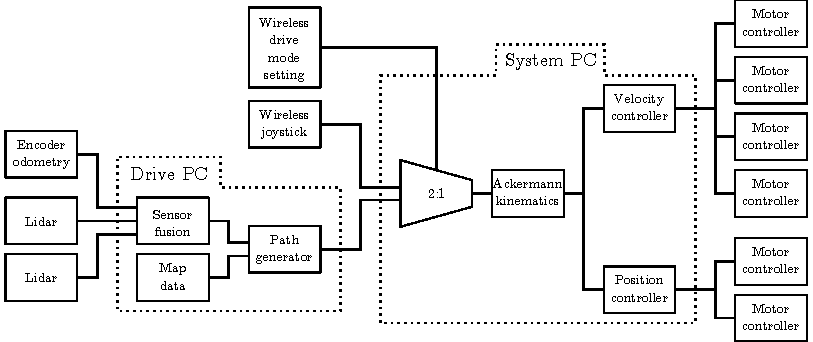
\includegraphics[width=\linewidth]{imgs/system_diagram/software.pdf}
        \caption{High level system diagram showing software architecture in terms of the manual and autonomous drive system.}
        \label{fig:system_diagram_software}
    \end{figure}

    A computer dedicated to processing sensing data related to navigation is connected to the platform's ``System PC'' via Ethernet.
    The open source Robotic Operating System (ROS) is used to facilitate communicate between the two computers.
    Not only is ROS used for inter-computer communication, but also within separate software nodes running on the same machine.
    Figure \ref{fig:system_diagram_software} shows the flow of data from various sources to the motor controllers.
    For simplicity it omits interface nodes, those used solely to interface the device to the ROS network.

    To maximise code reusablility, each device on the platform has its own node dedicated to publishing device data or subscribing to generated device commands.
    Examples of such devices are CAN adapters, motor controllers, wireless controllers, lidar, encoders.
    Nodes are also used to transform or perform calculations on available data as well as pass it between nodes written in either C++ or Python.

    In addition to the drive commands generated by the ``Drive PC'', a safety rated wireless controller lets the operator generate commands by joystick.
    The controller also has a mode selector that selects which commands are fed through to the motor drivers.
    An emergency stop button on the controller means that the platform can be stopped at any time.


\section{Autonomous Driving}
\label{sect:autonomous}
    Using the row following algorithm developed for sensor testing, map based autonomous navigation of a kiwifruit orchard demonstrated with two additions to the software.
    These additions were the detection of a row's end and a method for turning between rows.
    Using the developed navigation approaches, the platform presented here was able to navigate an orchard block unassisted.

    Detection of the end of a row was made by detecting a minimum volume of free space above the multi-layer lidar.
    This equates to the lidar searching for a lack of canopy above the robot.
    This makes use of the multi-layer lidar, where layers above the horizontal are used as an `absence of canopy' detector.

    Turns between rows were performed by driving a sequence of set curvature movements while performing obstacle avoidance.
    The set movements were recorded in a map file which were carried out by the platform on a turn-by-turn basis.
    A turn sequence would have the platform drive at a given angle for a given distance or until a given turn angle had been reached.
    Each row turn could contain any number of turn sub-manovours.
    On completion of the turn, the row following mode was entered which then guides the platform through the row.

    Figure \ref{fig:suzy_turning} shows the platform performing a row-end turn under autonomous control.

    \begin{figure}[htb]
        \centering
        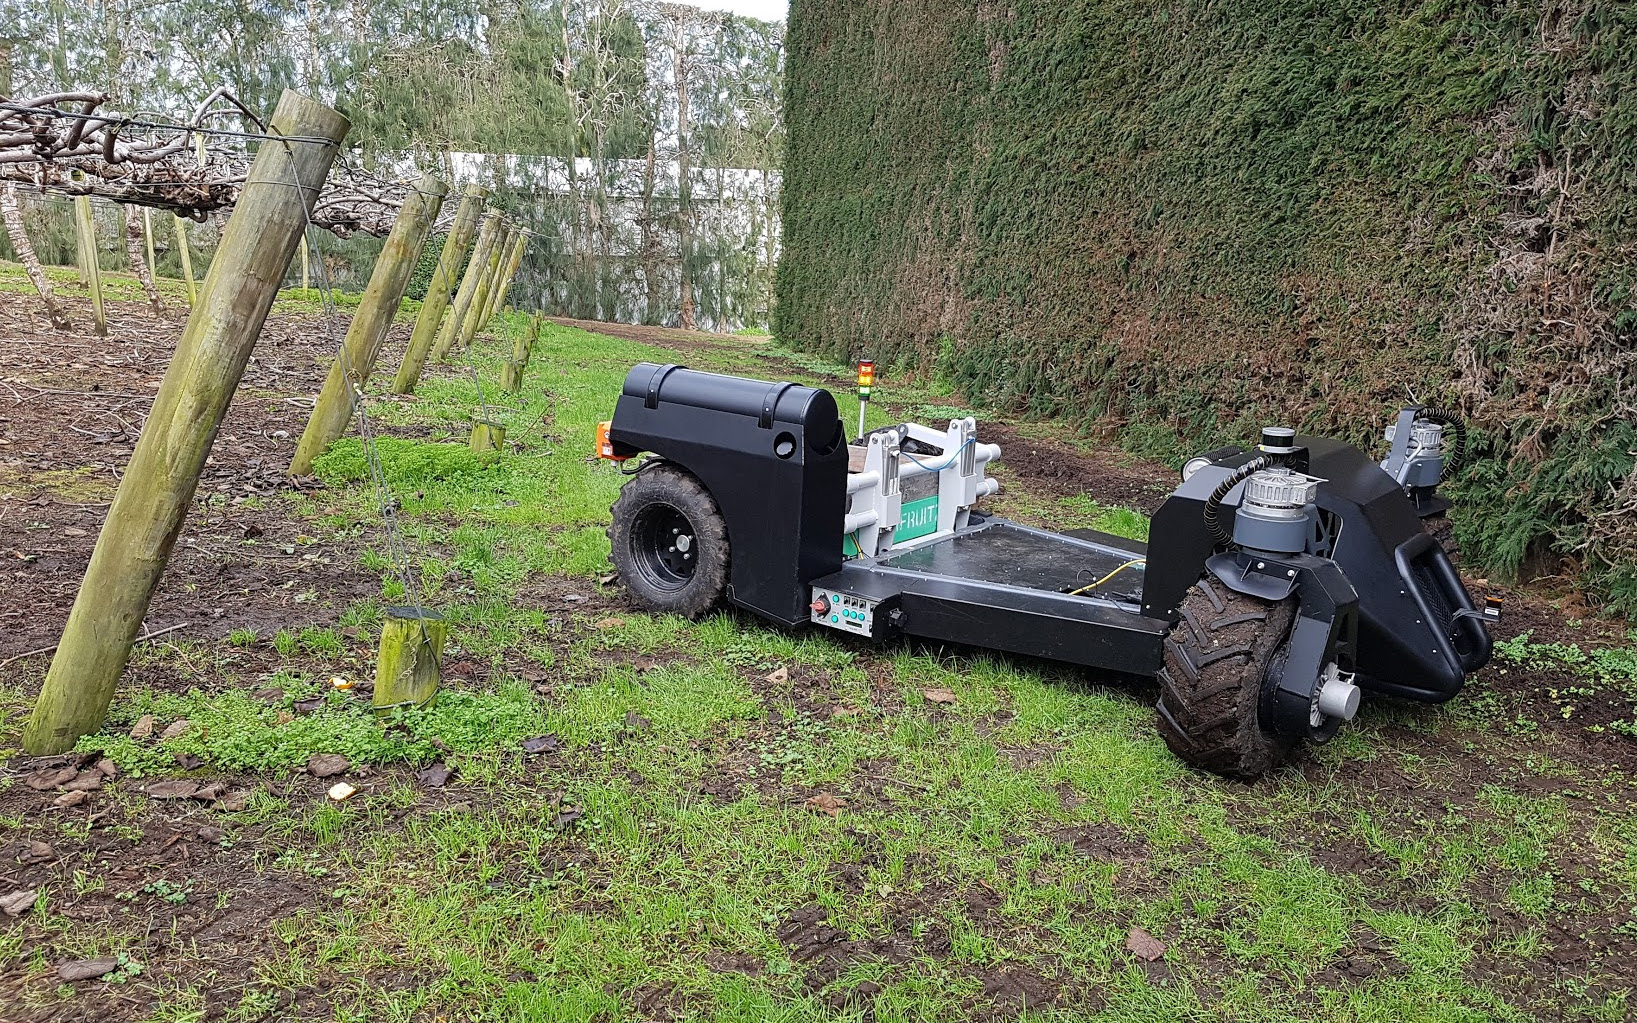
\includegraphics[width=\linewidth]{imgs/photos/suzy_turning.jpg}
        \caption{
            Photo showing the platform performing a row-end turn
        }
        \label{fig:suzy_turning}
    \end{figure}


\section{Conclusion}
    In this work, a platform designed specifically for driving through pergola style kiwifruit orchards has been presented.
    The platform has the capability to carry payloads of \SI{600}{\kilo\gram} through these orchards without performance degradation.
    Sensors suitable for autonomous navigation have been selected, trialled and demonstrated as being useful as a means of navigating in this environment.
    Convolutional neural networks applied to monocular image data proved to be a promising technique for row navigation.
    By processing multi-layer lidar data, the platform was able to sucessfully and reliably navigate an entire orchard block without intervention.


\section*{Acknowledgements}
This research was supported by the New Zealand Ministry for Business, Innovation and Employment (MBIE) on contract UOAX1414.
The authors acknowledge contributions from Phillip Ross, Gordon Neshausen, Josh Barnett and Erin Simms in the design and fabrication of the platform.

%% The Appendices part is started with the command \appendix;
%% appendix sections are then done as normal sections
%% \appendix

%% \section{}
%% \label{}

%% References
%%
%% Following citation commands can be used in the body text:
%%
%%  \citet{key}  ==>>  Jones et al. (1990)
%%  \citep{key}  ==>>  (Jones et al., 1990)
%%
%% Multiple citations as normal:
%% \citep{key1,key2}         ==>> (Jones et al., 1990; Smith, 1989)
%%                            or  (Jones et al., 1990, 1991)
%%                            or  (Jones et al., 1990a,b)
%% \cite{key} is the equivalent of \citet{key} in author-year mode
%%
%% Full author lists may be forced with \citet* or \citep*, e.g.
%%   \citep*{key}            ==>> (Jones, Baker, and Williams, 1990)
%%
%% Optional notes as:
%%   \citep[chap. 2]{key}    ==>> (Jones et al., 1990, chap. 2)
%%   \citep[e.g.,][]{key}    ==>> (e.g., Jones et al., 1990)
%%   \citep[see][pg. 34]{key}==>> (see Jones et al., 1990, pg. 34)
%%  (Note: in standard LaTeX, only one note is allowed, after the ref.
%%   Here, one note is like the standard, two make pre- and post-notes.)
%%
%%   \citealt{key}          ==>> Jones et al. 1990
%%   \citealt*{key}         ==>> Jones, Baker, and Williams 1990
%%   \citealp{key}          ==>> Jones et al., 1990
%%   \citealp*{key}         ==>> Jones, Baker, and Williams, 1990
%%
%% Additional citation possibilities
%%   \citeauthor{key}       ==>> Jones et al.
%%   \citeauthor*{key}      ==>> Jones, Baker, and Williams
%%   \citeyear{key}         ==>> 1990
%%   \citeyearpar{key}      ==>> (1990)
%%   \citetext{priv. comm.} ==>> (priv. comm.)
%%   \citenum{key}          ==>> 11 [non-superscripted]
%% Note: full author lists depends on whether the bib style supports them;
%%       if not, the abbreviated list is printed even when full requested.
%%
%% For names like della Robbia at the start of a sentence, use
%%   \Citet{dRob98}         ==>> Della Robbia (1998)
%%   \Citep{dRob98}         ==>> (Della Robbia, 1998)
%%   \Citeauthor{dRob98}    ==>> Della Robbia


%% References with bibTeX database:

\bibliographystyle{model5-names}
\bibliography{bibliography_jamie,bibliography_mark}


%% Authors are advised to submit their bibtex database files. They are
%% requested to list a bibtex style file in the manuscript if they do
%% not want to use model5-names.bst.

%% References without bibTeX database:

% \begin{thebibliography}{00}

%% \bibitem must have one of the following forms:
%%   \bibitem[Jones et al.(1990)]{key}...
%%   \bibitem[Jones et al.(1990)Jones, Baker, and Williams]{key}...
%%   \bibitem[Jones et al., 1990]{key}...
%%   \bibitem[\protect\citeauthoryear{Jones, Baker, and Williams}{Jones
%%       et al.}{1990}]{key}...
%%   \bibitem[\protect\citeauthoryear{Jones et al.}{1990}]{key}...
%%   \bibitem[\protect\astroncite{Jones et al.}{1990}]{key}...
%%   \bibitem[\protect\citename{Jones et al., }1990]{key}...
%%   \harvarditem[Jones et al.]{Jones, Baker, and Williams}{1990}{key}...
%%

% \bibitem[ ()]{}

% \end{thebibliography}

\end{document}

%%
%% End of file `elsarticle-template-5-harv.tex'.
